\subsection{Overview}

The data processing done by the summarisation tool is split into three stages: preparing the data for processing, extracting the associations between devices, and matching these association to find encounter between mobile devices. The data preparation stage simply consists of unzipping the input files and piping them to the next stage. The software component used for extraction of associations depends on the format of the input, however both of the implemented association extraction processes will output a temporary file of exactly the same format. This format can be read by the stage three process which finds the encounters between associations, it takes a temporary file as input and gives output as specified in the 'Design' section of this document.

\begin{figure}[h]
    \centering
    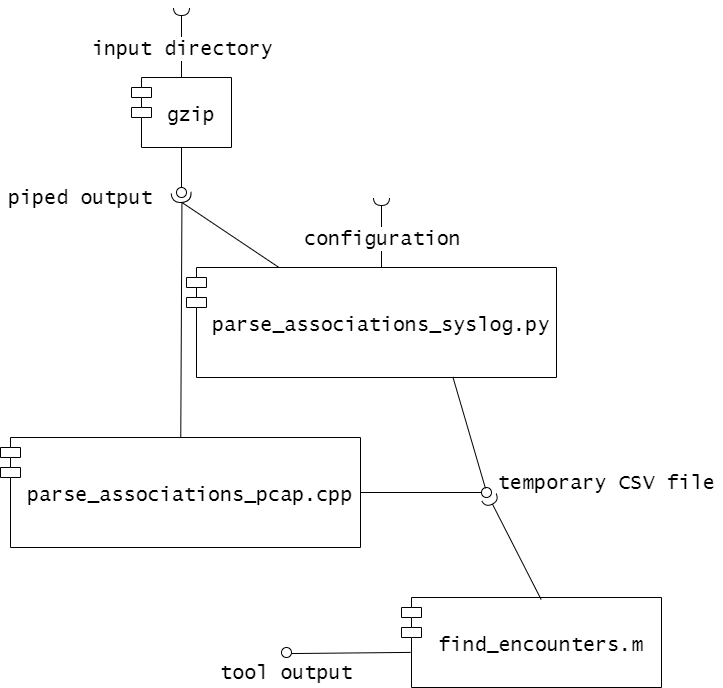
\includegraphics[width=0.8\textwidth]{component_diagram.png}
    \caption{This figure shows the different software components involved in the summarisation tool, and how they interface with each other. This is a high level representation of the system and shows no detail regarding how each component and interface works.}
    \label{fig:component_dia}
\end{figure}

Figure \ref{fig:component_dia} shows how the components of the summarisation tool are connected. There are separate association extraction components for each input type. As long as the correct interfaces are used for input and output it is a simple matter to connect a new program to parse and extract associations from a different input format.

\subsection{Stage One; Decompressing Files}

The datasets downloaded from the CRAWDAD site are initially compressed (as gzip files). A directory of compressed pcap files can be given as a parameter to the summarisation script. Each file in the given directory will be individually decompressed using gzip and piped into the first stage of the processing. This unfortunately causes associations which span multiple pcap files to be split at the temporal boundaries of the files.

\subsection{Stage Two; Extracting Associations}

Libpcap is a library written in C/C++ which provides functions for the analysis of network traffic, including reading and extracting information from pcap files such as those produced in tcpdump traces. Tcpdump was the utility used to capture the CRAWDAD dartmouth dataset on which this project is initially focused. There are several wrappers of libpcap written for different languages such as pycap \cite{pynetwork2019} for Python and jpcap \cite{charles2013}. These are generally not very regularly maintained and have very little documentation compared to Libpcap with C/C++. When initially reading in pcap files as input C++ will be used to extract the necessary information. In this stage of processing only information about the times of associations and MAC addresses of involved devices should be kept. Most of the processing will be done in subsequent stages, the main aim of this stage is to remove as much unnecessary information as possible, and to convert into an appropriate format for the next stage.

In this stage of processing a hash map of ongoing associations is built up during the reading of all packets from a pcap file. The map is updated every time a packet is read which signals the beginning of an association or the end of one. In the case of the beginning of an association, the map is updated by setting the MAC address pair to the two addresses between which the packet is sent (this is used as the key), and start and end times of the association are set to be the timestamp on the packet. Every time that a packet is read between a pair of devices the end time of the pairs current association is updated to the packets timestamp. Each packet is also checked to find whether the destination node of the pair is an access point. Since packet-specific information will be discarded after this stage it is necessary to identify access points with a flag. When the association ends, the values stored in the map are output in string delimited by commas. The values which are output are the source and destination MAC addresses, and start and end times of the association, and a flag (0 or 1) value identifying whether the destination device is an access point. This output is used as input in the subsequent processing stage.

\subsection{Stage Three; Finding Encounters} 

\begin{figure}[h]
    \centering
    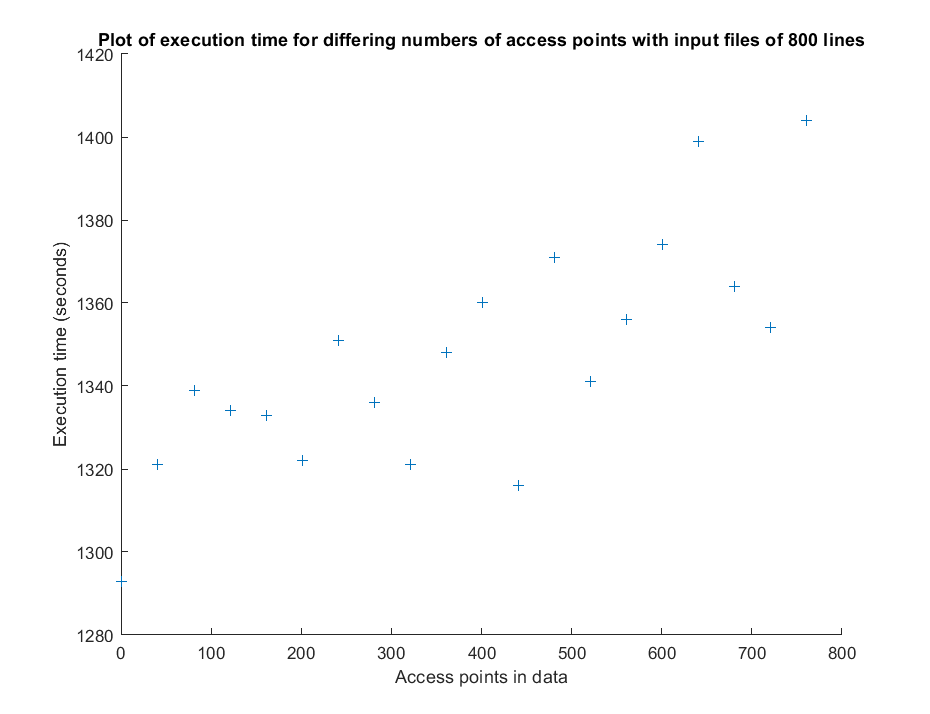
\includegraphics[width=\textwidth]{ap_vs_time.png}
    \caption{This figure shows the dependence of execution time on the number of access points in a file of associations for a file length of 800 lines. The files used as input to the MatLab code for this evaluation were fabricated to include specific numbers of distinct access point IDs. A roughly linear positive correlation is seen between the number of access points and the execution time.}
    \label{fig:AP_vs_time}
\end{figure}

The third stage of processing is written using MatLab. This decision was made due to the efficiency of the MatLab language when manipulating large tables of data (such as are used during this project) and my previous experience with the language in comparison to others similar such as Mathematica or Maple. Consideration was also given to continuing to develop this stage of processing using C++, similarly to the previous stage. This could potentially increase the efficiency and speed up processing time, however my familiarity with C++ is fairly limited and therefore the efficiency gained would likely not be worth the cost in development time by using C or C++.\\\\
This stage of processing has three main aims, firstly to extract a list of access points. Having a list of access points is important since encounters need to occur through access points (as described in the `Design' section). The second aim is to match up the timings of associations between mobile nodes and access points such that encounters can be identified. The final aim is to then find the average duration and frequency of encounters between each distinct pair of mobile nodes. 

\begin{figure}[h]
    \centering
    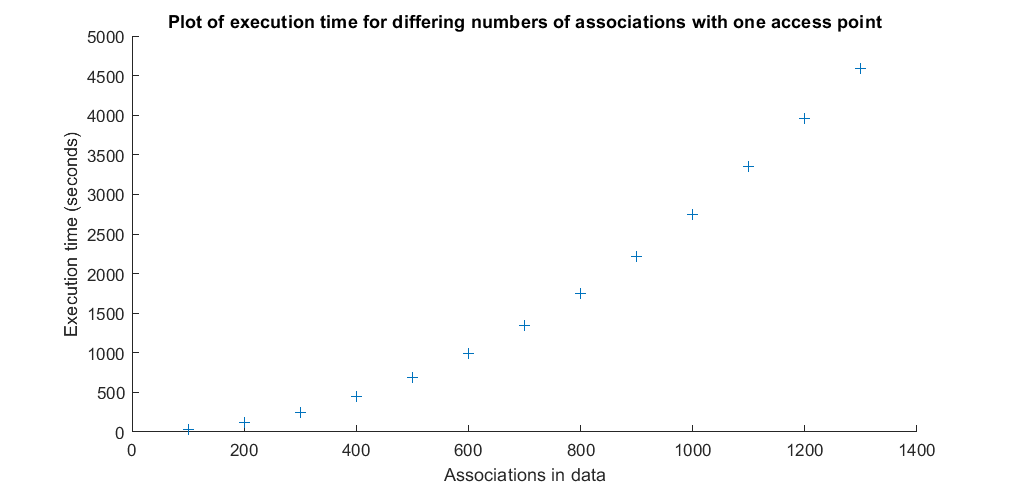
\includegraphics[width=\textwidth]{time_vs_lines.png}
    \caption{This figure shows the dependence of execution time on the number of associations in the intermediate file. Results are mean values averaged over ten iterations of each number of assciations. The files used as input to the MatLab code for this evaluation were fabricated to include specific numbers associations and a static number of access points. A power two positive correlation is seen between the number of associations and the execution time.}
    \label{fig:lines_vs_time}
\end{figure}

Initially the implementation of this stage of processing became drastically slower at high numbers of access points, this issue has been solved such that an almost linear behaviour in execution time if measured as the number of access points increases (shown in figure \ref{fig:AP_vs_time}) whereas in figure \ref{fig:lines_vs_time} it can be seen that the execution time still increases with a quadratic curve as the line length of the intermediate associations file increases. The limiting factor is now the total length of the input file for this stage of processing.

